%! root = ../../main.tex

\subsection{Алгоритм нахождения контрольной суммы}

Реализуемый метод защиты заключается в том, что программа подсчитывает
контрольную сумму участка кода и сравнивает с эталонным значением. Если
контрольные суммы не совпадают программа должна изменить свое поведение с
учетом того, что она находится по угрозой взлома.

Алгоритм нахождения контрольной суммы должен быть быстрым, чтобы по задержке
нельзя было определить место в программе, где осуществляется проверка. Также
алгоритм не должен хранить в памяти большое количество промежуточных данных, так
как это тоже упрощает нахождение блока защиты.

Исходя из этих условий был разработан алгоритм, блок-схема которого представлена
на рисунке \ref{fig:algorithm}. Данный, алгоритм основан на том факте, что поля
в таблице релокаций отсортированы по возрастанию. Алгоритм состоит из главного
цикла, в котором суммируется каждый байт секции, кроме тех случаев, когда адрес
проверяемого байта есть в таблице релокаций (в этом случае этот байт и три
следующих за ним игнорируются). Если при проверке окажется, что адрес
проверяемого байта больше, чем значение поля таблицы релокаций, то берется
следующее поле. Таким образом полученный алгоритм имеет линейную сложность.

В данном подходе игнорируется указанный в поле таблицы релокации тип смещения.
Это сделано для того, чтобы код алгоритма подсчета контрольной суммы имел
минимальный размер. 

Также перед началом алгоритма необходимо найти и сохранить в памяти адрес начала
проверяемой секции, размер проверяемой секции, адрес, по которому размещена
таблица базовых релокаций, и размер таблицы. В реализованном алгоритме данные
значения хранятся в стеке.

%\newgeometry{top=5mm, bottom=20mm, left=5mm, right=5mm}
\begin{figure}[h!]
  \centering
  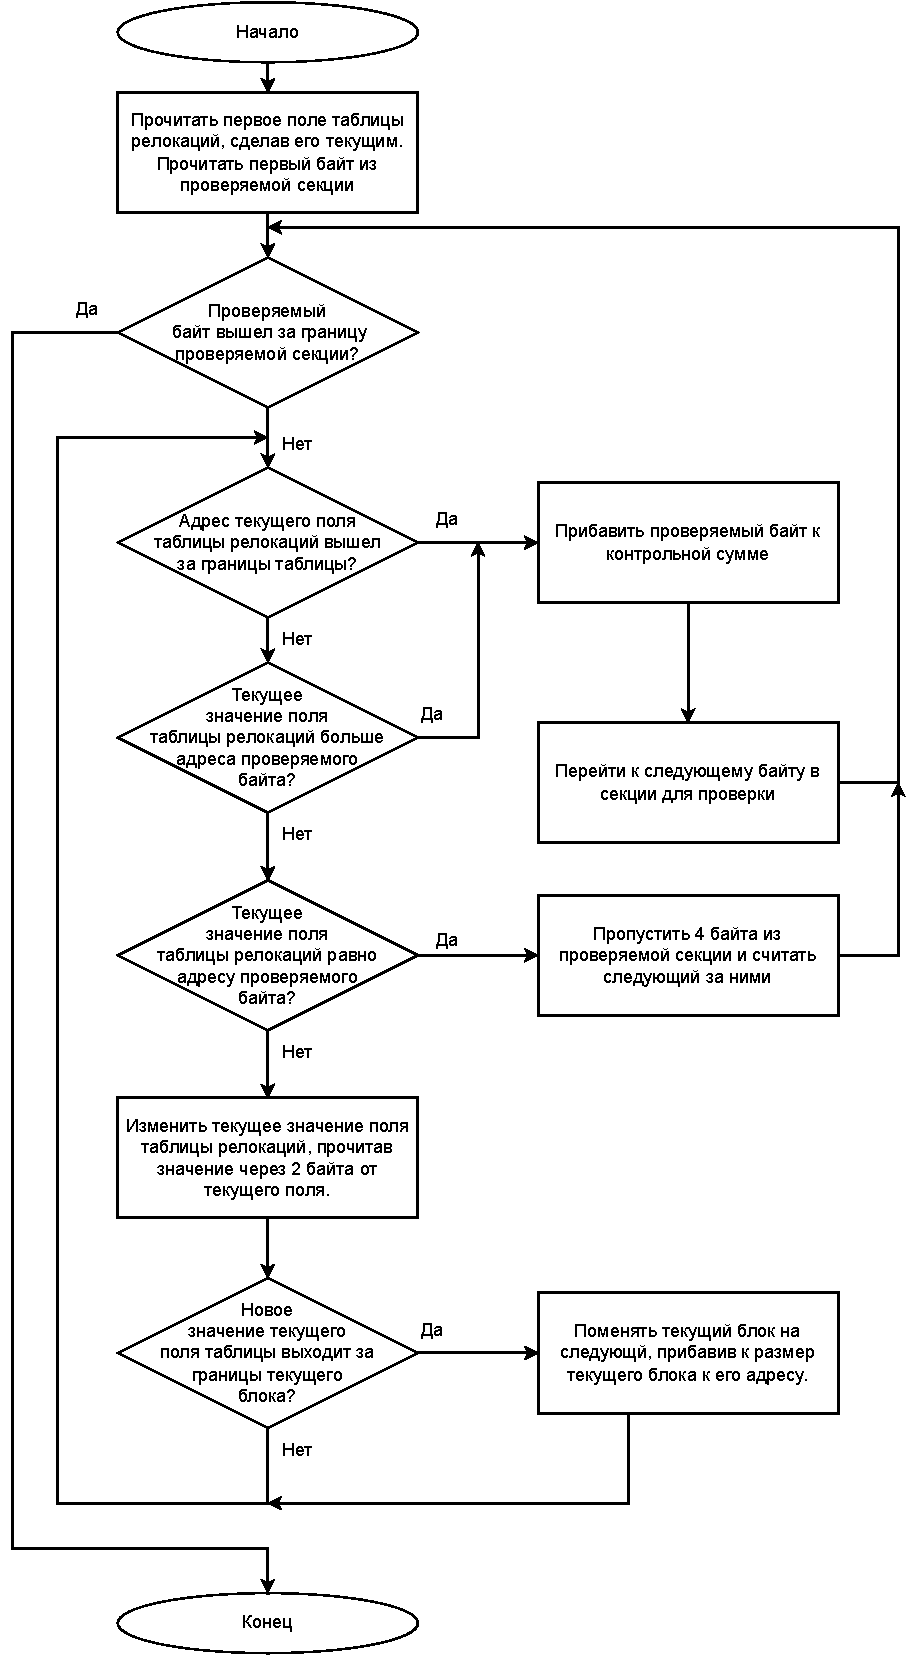
\includegraphics[height=\textheight]{algorithm.pdf}
  \caption{Блок-схема алгоритма по нахождению контрольной суммы}
  \label{fig:algorithm}
\end{figure}
%\restoregeometry
